\chapter {绪论}
\label{chp:intro}

\section{研究背景}

% With the growing attention of mobile markets, Android has accounted for 85.9\% of global market share~\cite{Gartner_report}. Over 1.5 million apps were released within 2017 alone.
% Along with the booming of Android markets is the flourish of the mobile underground industry. \emph{Fake apps}, i.e., apps without official certificates, account for a major part of such underground industry.
% Specifically, we consider fake apps as those who simulate the corresponding official ones or look almost the same as their official correspondences, with ultimate goal to elicit download or manifest malicious behaviors.
% Early observation reveals fake apps come in two different forms.
% The first category is called \texttt{imitators}, a group of apps with similar names or functionalities to their official correspondences so that users are fooled to download them.
% While imitators are just similar to official apps, \texttt{imposters}~\cite{Andow2016ASO} refer to the category of apps that have exactly the same metadata with their official correspondences, for example, they may have the same names, icons, or version numbers, some of the imposters are even made by repackaging official apk files directly.
随着移动市场于近年逐渐兴起,Android系统作为一个主流的移动端操作系统也在蓬勃发展。
根据数据分析机构StatCounter的资料显示,从发布之日起,Android的市场占有率就在逐年稳步增长。截至2020年,Android系统已经占据了74.3\%的全球移动端市场份额~\cite{MobileOSMktShare}。
与此同时,Android应用的数量也伴随着Android市场的蓬勃发展节节攀高。
仅看Android官方的应用商店Google Play,其在2017年一年中就新上架了近一百万个可供下载的应用程序。
虽然因为各种原因,Google Play上的应用数量在2018年有所回落,但如\autoref{fig:app_number}所示,应用市场上目前仍有近三百万个可用的应用程序,Android应用市场依然充满活力~\cite{StatistaAppNumber}。

\begin{figure}[htbp]
	\centering
	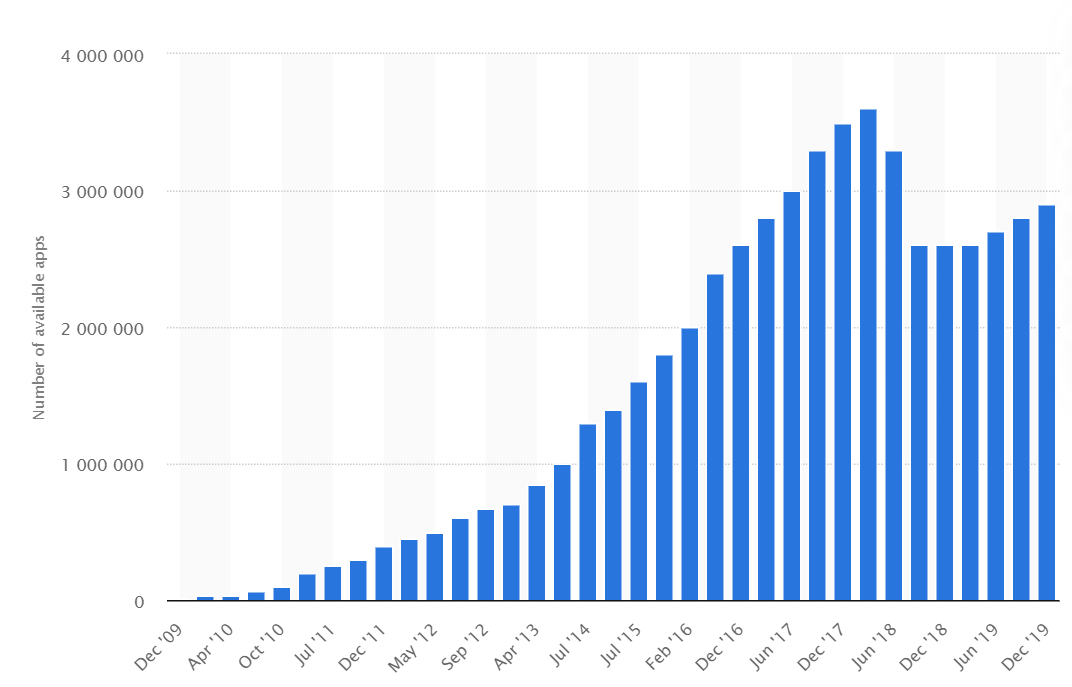
\includegraphics[width=0.9\textwidth]{./Figures/edwin-intro-app-number.png}
	\caption{Google Play 应用商店架上应用总数变化趋势}
	\label{fig:app_number}
\end{figure}

伴随着应用数量爆发式增长的,还有欣欣向荣的移动黑灰产。
\emph{仿冒应用}构建了移动黑灰产工业链中十分重要的一环。
本文提及的仿冒应用指代模仿市面上热门的应用、甚至外观与热门应用相差无几的移动应用,其目的是诱导用户下载以赚取流量,甚至是窃取用户信息、触发有害行为从而盈利。
根据的前期观察,我们发现仿冒应用以两种不同的形式出现。
第一类为\texttt{模仿应用},这类应用具有和原版热门应用相似的外观(比如名字、图标等),诱导用户下载。
而第二类,\texttt{高仿应用}~\cite{Andow2016ASO, luo2016repackage},已不单单是与原应用``相似''了,这类应用采用和原应用一模一样的外观,乃至连版本号都相同,其中的部分应用就是直接通过对原应用重打包做成的。

% Such fake apps pose significant problems to not only the official developers' interest but also the end users' right.
% For example, when users try to search an app for installation in market, multiple fake apps with similar names or icons will be retrieved at the same time.
% As a result, the user experience of app searching and downloading is greatly affected by the fake apps in real world.
这些仿冒应用不仅大大损害了原应用开发者的利益,也侵犯了用户的权益。
我们可以假设一个十分普遍的场景:当用户尝试通过应用市场搜索安装一个应用,应用市场往往会返回多个无论是名字或是图标都十分相像的结果,在这种情况下,用户十分有可能安装一个仿冒应用。
就算用户最后通过某些途径安装上了原版应用,也浪费了时间和人力成本,遑论某些仿冒应用中潜藏着恶意行为,一旦被触发就会对用户造成更大的损害。
于是,用户搜索与下载应用时的安全和体验就被仿冒应用严重影响了。

% Even worse, as the doorsill to develop an app has been set low, the cost to develop a fake app is much lower than what it takes to develop a desktop program, providing an ideal hotbed for the underground industry to thrive on~\cite{wasserman2010software}. Moreover, the flexibility of Android app implementation~\cite{storydroid} contributes the fake apps' complexity.
更糟糕的是,随着开发移动应用的门槛逐渐下降,开发一个仿冒应用的成本已经远低于开发一个桌面级应用所需的成本,这为地下产业涌入移动端发展提供了绝佳的温床~\cite{wasserman2010software}。
此外,移动应用功能在实现上的灵活性~\cite{storydroid}也增加了仿冒应用的复杂度,让分析移动应用变得更加困难。

% Despite the ubiquity, little is known about fake apps and their ecosystem -- their common characteristics, the number of fake apps at large, their production process and speed, and their evasive strategies, etc.
% Most research studies to date show greater interests on malware detection techniques~\cite{chen2016stormdroid,chen2018automated, chen2016towards, fan2016poster}. To the best of authors' knowledge, there exists no work in understanding fake apps, and their ecosystem.
% Similarly, we witness the same deficiency in industry.
% Most attention in analysis and threat reports focuses on malicious apps while neglecting the fake apps~\cite{McAfee_mobile_thread_report}.
% On the other hand, the knowledge gained from desktop era regarding malicious or fake software are of less use, due to differences in operating system properties~\cite{yin2007panorama}.
尽管如今仿冒应用随处可见,我们对仿冒应用和他们的生态却依然知之甚少——他们有何共同特征、数量多少、迭代速度如何、以及他们如何规避应用市场检测等问题依然有待解答。
遗憾的是,如今关于移动应用的学术研究大多关注于恶意应用的检测技术~\cite{chen2016stormdroid,chen2018automated, chen2016towards, fan2016poster}。据我们所知,目前还未有任何关于仿冒应用或其生态系统的研究。
类似地,工业界中也鲜见关于仿冒应用的课题。多数分析与威胁报告都聚焦于恶意应用上,忽略了仿冒应用~\cite{McAfee_mobile_thread_report}。
而在另一方面,由于底层、实现等各个层面上的差异,从桌面平台上获取的关于仿冒软件的知识也不能很好地用于了解移动端仿冒应用~\cite{yin2007panorama}。

\section{学术界研究现状}

% \subsection{Empirical studies on malware ecosystem}
\subsection{针对恶意应用生态系统的研究}

% 46 malware samples on various platforms are dissected to gain understanding on their incentive system as in a survey conducted by Felt et al.~\cite{Felt2011ASO}. Meanwhile, several strategies are proposed by them to defend again these type of malware.
% Zhou and Jiang~\cite{Zhou2012DissectingAM} gathered over 1,200 malware samples across major Android malware families, systematically characterizing their different natures including installation methods, activation mechanisms and how the payload is carried out.
% These researches help expand practitioners' horizon in terms of malicious app's behavior, but the insight they provide may not suit fake app identification well.
在Felt主导的一次研究~\cite{Felt2011ASO}中,研究人员仔细剖析了来自多个不同平台的46个恶意程序样本以了解这些样本的激励机制。该篇文献也揭示了这些样本的运行机制和行为策略,为后人抵御此类恶意行为提供参考。
另外,Zhou和Jiang~\cite{Zhou2012DissectingAM}搜集了来自多个主要恶意应用家族的、超过1,200个恶意应用样本,系统性地描绘了这批样本的不同性质,包括其安装手段、激活机制和其如何执行有效负载(实现恶意行为);在另一篇著作~\cite{zhou2012hey}中,他们提出了名为DroidRanger的系统,并成功地从5个应用市场的204,040个应用中找出了211个恶意应用。

这类研究帮助了从业者拓宽视野,使得从业者对恶意应用的行为更加了解。
然而正如上文提及,仿冒应用与恶意应用分属同一产业中的不同链条,针对仿冒应用的专门研究依然是有必要的。

% \subsection{Repackage detection}
\subsection{重打包应用检测}
\label{sec:repackaging}
% Prior work on repackage detection generally falls into five categories.
% The first one is based on apps' \textit{instruction sequences}, which uses fuzzy hashing techniques to extract the digest of apps, then calculates similarity between every two digests~\cite{DroidMOSS,Zheng2013DroidAnalyticsA}.
% The second one is based on \textit{semantic information}.
% CLANdroid~\cite{CLANdroid} detects similar apps through analyzing five semantic anchors (e.g., identifiers and Android APIs).
% The third kind leverages \textit{lib detection} methods.
% CodeMatch~\cite{CodeMatch} filters out libraries used in apps then compares the hash of their remnant.
% Wukong~\cite{Wukong} detects repackage apps in two steps, but that it processes the second step by using a counting-based code clone detection approach, instead of hash.
% ViewDroid~\cite{ViewDroid} picks out repackage apps by rebuilding and comparing the viewgraph of different apps, belongs to the forth kind which makes use of \textit{visualizes information}.
% The fifth kind applies \textit{graph theory} on measuring app similarity.
% DNADroid~\cite{DNADroid} calculate apps' similarity based on program dependency graph (PDG), while AnDarwin~\cite{AnDarwin} builds semantic vectors with PDG extracted from every methods.
% Centroid~\cite{Centroid} even constructs 3D-control-flow-graph (3D-CFG) for each method in an app and see how alike the centroid in different apps are.
重打包指恶意开发者对原应用解包、篡改内容之后再将应用重新打包的技术,重打包应用也属于移动黑灰产业范畴。
针对重打包检测的前人研究大致可划分为五个类别:

第一类是基于应用\textit{指令序列}的。这种方法使用模糊哈希的方法提取出应用的摘要信息,然后通过比对两两应用之间的摘要信息来获得应用之间的相似度~\cite{DroidMOSS, Zheng2013DroidAnalyticsA}。
第二类凭借\textit{语义信息}比对应用。如CLANdroid~\cite{CLANdroid}通过分析五种语义特征点(比如代码中的标识符和调用到的AndroidAPI等)。
第三类利用了\textit{第三方库检测}手段。CodeMatch~\cite{CodeMatch}筛选出应用中使用的第三方库代码后,计算并比对剩余部分代码的哈希值。
Wukong~\cite{Wukong}也分两步检测重打包应用,但与CodeMatch相比,其第二步使用了基于计数的代码克隆检测手段,而非基于哈希的技术。
ViewDroid~\cite{ViewDroid}通过重建和比对应用的视图来筛出重打包应用,这种技术属于第四类\textit{信息可视化}。
第五类依赖\textit{图论}衡量应用相似性。
DNADroid~\cite{DNADroid}基于应用的程序依赖图(Program Dependency Graph, PDG)来比对应用相似性,而AnDarwin~\cite{AnDarwin}则用从每个方法从提取的PDG构建出语义向量,再计算向量间相似度以检测重打包应用。
Centroid~\cite{Centroid}甚至为应用中的每个函数构建了三维控制流图(3-Dimensional Control Flow Graph, 3D-CFG),然后再将三位控制流图聚合,通过检测不同应用在控制图聚合后的质心位置判断应用间的相似程度。

% Each of these approaches has its own advantages and drawbacks, from the perspective of scalability and accuracy, which are beyond the topic in this article.
% One common they all do share, however, are that the verification step, without any exception, is based on certificate system.
% Once the illegal developers poison data with legal certificates through apps with vulnerable signature scheme, even the state of the art detecting approach can do nothing about it.
检测方法林林总总,在此不一一列举,从检测的准确性和可伸缩性上看,每种都均有优缺点,其并不在本文的讨论范围之内。
然而,他们全都有一个共同之处:在验证阶段,无一例外,都是基于证书系统进行的。
一旦非法开发者利用具有漏洞的证书签名机制,污染了实验中的部分应用数据,即使是最先进的重打包检测机制也无用武之地。

% \subsection{Empirical study on grayware}
\subsection{针对灰色应用的实证研究}

% Andow et al.~\cite{Andow2016ASO} proposed a study of grayware, in which 9 types of greyware are defined and triaged from data retrieved from google play. We referred the definition on \textit{imposter} from this article.
Andow等人曾发表过一篇针对灰色应用的研究文献~\cite{Andow2016ASO}。其中,他们从Google Play应用商店中采集了应用样本,并将样本分类,定义出了9种不同的灰色应用。
灰色应用即那些并非具有明显的恶意行为,但应用意图存疑、又或是会向系统申请过多权限的应用程序。
本文中对\texttt{高仿应用}的定义参考了这篇文献中的内容。

\subsection{应用评论相关研究}
近年来,除了对Android App本身的分析研究之外,有不少学者也把研究焦点投放在了应用市场的评论上。

Bin Fu等人在2013年发布了WisCom~\cite{fu2013people}——对于某个应用,将其历史评级和评论记录输入WisCom,系统在反馈应用评级变化的同时,也能告诉使用者为什么会受到恶评;
而Deguang Kong~\cite{kong2015autoreb}等人在2015年发布的AUTOREB则结合了NLP、机器学习技术和声誉系统,先提取用户在某款App的评论中提及到的与安全相关的内容,然后根据每个用户的可信度对该款App是否可能有危险行为进行分数计算,最后用机器学习技术对App进行分类,预测该款App是否会有危险行为。

另一方面,大量的前人工作~\cite{hernandez2019the, xie2014grouptie, zhu2014discovery, hu2019want, chen2017toward, xie2016you, hooi2016fraudar}揭示,很多应用市场都饱受虚假评论的困扰。
Rahman等人在2019年发布了一个关于虚假评论行为的实证研究~\cite{rahman2019art},在公开确认了这个产业链存在的同时,也对揭露了他们的行为模式、生存情况甚至是收入水平等方面的信息。


\section{论文研究意义}

前文的学术界研究现状,不仅反映出移动黑灰产业是目前的研究热点之一,更反映出移动黑灰产从业者无孔不入的特点。
为了保障正当开发者的利益与消费者的权益,我们需要对移动黑灰产有更全面、更深入的理解,从而更好地预防未知的威胁。
然而,现有研究提供的知识仍有空缺部分,仿冒应用部分正是缺口之一。
因此,我们首先需要搜集大量仿冒应用的信息,补全我们对移动黑灰产这一环节的认识。

为了达到这个目标,我们借助犇众信息的移动安全威胁数据平台Janus\footnote{\url{https://www.appscan.io/}}搜集并分析了大量应用样本,完成了一次大规模实证研究,对仿冒应用作出了较为全面的剖析,填补了本领域的研究空白。
通过收集仿冒应用在市场上获得的反馈,我们还进一步验证了仿冒应用和排名欺诈行为的关系,进一步地提供了关于仿冒应用生态的知识。


\section{论文研究内容}
本文的主要研究工作如下:
\begin{itemize}
	%				\setlength{\itemsep}{-5pt}
	\setlength{\itemsep}{1pt}
	\setlength{\parskip}{0pt}
	\setlength{\parsep}{0pt}

	\item{\bf 首次针对Android仿冒应用的大规模数据搜集}
	针对市面上最后欢迎的50款应用,我们从各个应用市场中收集了超过13万个应用样本数据,再从中筛选出了约5万个仿冒样本,完成了首次针对Android仿冒应用的大规模数据搜集。

	\item{\bf 对工业界中仿冒应用的实证研究}
	在大量工业界数据的支持下,我们进行了第一次针对Android仿冒应用的实证研究,补充了对移动黑灰产的研究空白。
	其具体从以下三个方面入手:
	\begin{itemize}
		\item 仿冒应用的基本特征
		\item 影响仿冒应用数量的因素
		\item 仿冒应用的发展轨迹
	\end{itemize}

	\item {\bf 基于真实案例发掘仿冒应用特征}
	之后,我们从样本信息中对数据进行挖掘,获得了几个真实案例。
	通过对案例的分析,我们进一步印证了前序测量中发现的结果与结论。

	\item {\bf 对仿冒应用评论的挖掘与分析}
	最后,我们进一步从应用评论出发,在试图从市场反应了解用户对仿冒应用的态度以外,也使用了两种不同方法探究了仿冒应用与近期研究热点之一——排名欺诈行为——之间的关联,以深化读者对仿冒应用生态的了解。

\end{itemize}


\section{研究中的困难与挑战}
在实证研究中,工作者通常都会遇到几点挑战:如何确定研究主体、如何收集数据、如何对数据进行有效处理。
在本研究中,对应的三点挑战可被整理如下:

1)	如何确定仿冒应用?

仿冒应用和正版应用是相对的概念。
我们选择了市面上最热门的50个应用,再搜集其对应的仿冒应用样本。
从应用中筛选出与热门应用外观相似或是相同的样本后,我们使用Android本身自带的证书机制,将获得样本的证书信息与原版应用的证书信息进行比对,从而鉴别出仿冒的样本。

2)	如何获得针对仿冒应用的大量数据?

数据搜集是科研工作中公认的难点。
本文想要提供一次全面的研究结果,除了搜集的目标应用需要由多样性之外,也必须获得不同应用市场上的数据,增加研究的代表性。
前文提及犇众信息的移动安全威胁数据平台Janus是一个数据整合平台。该平台每天从各大Android应用市场爬取应用样本入库,免去了我们要针对各个市场重新定制爬虫代码的麻烦。
结合网络爬虫技术,我们顺利从Janus搜寻到了超过15万条数据条目作为原始数据,其中每条数据条目代表Janus从应用市场上获得的一个应用样本。

3)	如何对大量的数据进行有效处理?

数据规模和处理效率一直是一对矛盾。
由于一条数据条目代表一个应用样本,要对超过15万个应用样本进行详尽分析,明显太耗费时间成本与计算成本;然而,如果只对样本进行简单处理,获得的分析结果就不够全面和深入。
在尽量确保分析全面性的前提下,对于每个样本,我们只抽取关键信息进行分析,而不对整个应用的代码进行详尽的静态分析或者动态分析,以节省时间与计算成本。


\section{本文组织结构}
本文共分为七章,环绕着本次实证研究的数据搜集和分析过程、分析结果展开,各章节内容如下:

\fullref{chp:intro} 主要介绍了本文的研究背景、相关工作、研究意义、研究内容及本文遇到的困难与挑战。

\fullref{chp:background} 介绍了Android应用的构建流程、Android安全证书机制、应用市场与黑灰产业的关系和一些已知的移动黑灰产知识。

\fullref{chp:dataCollection} 提供了本篇研究的概览,解释了数据收集流程。包括收集了什么数据、收集数据的分步解释和收集到的数据概览。

\fullref{chp:discoveries} 从多个视角分类提出并解说针对这批仿冒应用数据得到的发现。三个视角包括仿冒应用特征、影响仿冒应用数量的因素和仿冒应用的发展轨迹,每个视角都被进一步分解成了多个不同的研究问题。

\fullref{chp:casestudy} 结合上一章中提出的各个发现,挑出数据中具有代表性的一些案例进行案例分析,以案例进一步佐证分析结果的正确性。

\fullref{chp:feedback} 在前文基础上,从应用市场上搜集了部分仿冒应用的评论进行分析,并使用了近年来学界对排名欺诈行为的研究方法对仿冒应用的评论进行了排查,以检测仿冒应用和排名欺诈行为之间是否存在关联。

\fullref{chp:future} 对本文工作进行总结,并对下一步工作进行展望。
